%%%%%%%%%%%%%%%%%%%%%%%%%%%%%%%%%%%%%%%%%
% University Assignment Title Page 
% LaTeX Template
% Version 1.0 (27/12/12)
%
% This template has been downloaded from:
% http://www.LaTeXTemplates.com
%
% Original author:
% WikiBooks (http://en.wikibooks.org/wiki/LaTeX/Title_Creation)
%
% License:
% CC BY-NC-SA 3.0 (http://creativecommons.org/licenses/by-nc-sa/3.0/)
% 
% Instructions for using this template:
% This title page is capable of being compiled as is. This is not useful for 
% including it in another document. To do this, you have two options: 
%
% 1) Copy/paste everything between \begin{document} and \end{document} 
% starting at \begin{titlepage} and paste this into another LaTeX file where you 
% want your title page.
% OR
% 2) Remove everything outside the \begin{titlepage} and \end{titlepage} and 
% move this file to the same directory as the LaTeX file you wish to add it to. 
% Then add \input{./title_page_1.tex} to your LaTeX file where you want your
% title page.
%
%%%%%%%%%%%%%%%%%%%%%%%%%%%%%%%%%%%%%%%%%
%\title{relatorioEDA2}
%----------------------------------------------------------------------------------------
%	PACKAGES AND OTHER DOCUMENT CONFIGURATIONS
%----------------------------------------------------------------------------------------

\makeindex
\documentclass[a4paper,12pt,headings=small]{article}
\usepackage[english]{babel}
\usepackage[export]{adjustbox}
\usepackage[utf8x]{inputenc}
\usepackage{amsmath}
\usepackage{graphicx}
\usepackage[colorinlistoftodos]{todonotes}
\usepackage{placeins}
\usepackage{makeidx}
\usepackage[left=2.5cm,right=2.5cm,top=2.5cm,bottom=2.5cm,a4paper]{geometry}
\usepackage{blindtext}
\setlength\footskip{1cm}

\begin{document}

\begin{titlepage}

\newcommand{\HRule}{\rule{\linewidth}{0.5mm}} % Defines a new command for the horizontal lines, change thickness here

\center % Center everything on the page




 %----------------------------------------------------------------------------------------
%	LOGO SECTION
%----------------------------------------------------------------------------------------


\includegraphics[scale=0.5]{uevora.png}\\[0.5cm] % Include a department/university logo - this will require the graphicx package

%----------------------------------------------------------------------------------------
 
%----------------------------------------------------------------------------------------
%	HEADING SECTIONS
%----------------------------------------------------------------------------------------

\textsc{\LARGE Universidade de Évora}\\[1.5cm] % Name of your university/college
\textsc{\Large Disciplina de Estruturas de Dados e Algoritmos II}\\[0.5cm]

% Major heading such as course name
%\textsc{\large Minor Heading}\\[0.5cm] % Minor heading such as course title

%----------------------------------------------------------------------------------------
%	TITLE SECTION
%----------------------------------------------------------------------------------------

\HRule \\[0.4cm]
{ \huge \bfseries Caça aos Erros - Corrector Ortográfico}\\[0.4cm] % Title of your document
\HRule \\[1cm]
 

\includegraphics[scale=0.65]{dictionary.png}\\[1cm]
%----------------------------------------------------------------------------------------
%	AUTHOR SECTION
%----------------------------------------------------------------------------------------

\begin{minipage}{0.4\textwidth}
\begin{flushleft} \large
\emph{Autores:}\\
Ricardo \textsc{Fusco}, 29263\\
Miguel \textsc{Casco}, 28966
\end{flushleft}
\end{minipage}
~
\begin{minipage}{0.4\textwidth}
\begin{flushright} \large
\emph{Professor:} \\
Vasco \textsc{Pedro}
\end{flushright}
\end{minipage}\\[2cm]

% If you don't want a supervisor, uncomment the two lines below and remove the section above
%\Large \emph{Author:}\\
%John \textsc{Smith}\\[3cm] % Your name

%----------------------------------------------------------------------------------------
%	DATE SECTION
%----------------------------------------------------------------------------------------

{\large 8 de Junho, 2014}\\[1cm] % Date, change the \today to a set date if you want to be precise
 

\vfill % Fill the rest of the page with whitespace

\end{titlepage}

\newpage
\thispagestyle{empty}
\renewcommand\contentsname{Índice}
\tableofcontents
\newpage
\renewcommand\listfigurename{Lista de Figuras}
\listoffigures
\newpage

\printindex
\section{Introdução}

\FloatBarrier

	No âmbito da unidade curricular de Estruturas de Dados II pretende-se, através das estruturas e algoritmos abordados ao longo das aulas de EDA nomeadamente as tabelas de Hash, algoritmos de sort, etc, criar um corrector ortográfico simples que gera como output no terminal as k palavras que constituem um erro, o número de ocorrências de cada erro e as linhas onde se observam tais ocorrências. Para tal é necessário processar um dicionário, fornecido pelo professor, que irá ser redireccionado para o standard input do programa e servir como base para criar a estrutura em disco (Hashtable). Após criada a estrutura em disco será necessário ir carregando blocos do ficheiro em disco para a memória, conforme necessário, à medida que se vai processando cada palavra do ficheiro com o texto que pretendemos corrigir que irá ser redireccionado para o standard input. A estrutura onde vão ser inseridos os erros é uma hashtable em memória usando um array de Erros, esse array irá no fim ser ordenado com um algoritmo de sort para que fique em ordem decrescente do numero de ocorrências e, caso tenham número igual de ocorrências, ficarão por ordem crescente de valor lexicográfico das palavras. As hashtables usadas são de acesso Linear.

\newpage

\section{Desenvolvimento}
\FloatBarrier

\subsection{Estruturas}

\subsubsection{Hashtables}

Como já foi referido anteriormente, para realizar este trabalho foram usadas HashTables de acesso linear.\\

Foi usada uma hashtable fechada usando um array de elementos, em que cada elemento é composto por um array de char's correspondente à palavra nessa posição e um inteiro que serve como "flag" para saber se essa posição da hashtable está a ser usada (1) ou não (0), poderia ter sido utilizado um booleano, mas foi usado um inteiro para que cada elemento tivesse exactamente 32 bytes para impedir que houvessem problemas ao carregar um bloco de elementos nomeadamente ter elementos entre 2 páginas que iria resultar num número maior de páginas acedidas visto que teria que aceder a duas páginas diferentes para carregar apenas um bloco. Assim, desta maneira, é garantido que cada bloco contém 4096 bytes, o tamanho de uma página. 

Na implementação que fizemos de hashtables não implementámos o rehash pois para este trabalho não nos interessa que a hashtable aumente de tamanho, interessa-nos sim que esta mantenha o seu tamanho tornando desnecessário o rehash.\\

Na figura seguinte pode-se observar um pequeno exemplo de como está estruturada a hashtable.

\begin{figure}[ht]
\centering
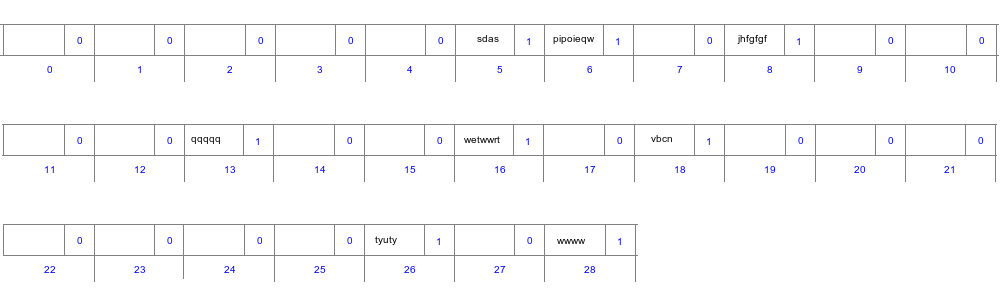
\includegraphics[scale=0.45]{hashTable.jpg}\\[1cm]
\caption{Exemplo Tabela Hash (Elementos)}
\label{fig:minipage1}
\end{figure}

O trabalho está dividido em 2 partes, a parte do programa de criação do dicionário em disco e a parte do corrector ortográfico em si.

A primeira coisa que é feita na primeira parte do trabalho é a criação de um novo ficheiro vazio com um nome que é especificado por nós (dic.data), de seguida são colocados Elementos em cada posição da hashtable em disco fazendo a escrita elemento a elemento (32 em 32 bytes), sendo que o elemento que está a ser escrito teve os seus campos previamente inicializados a 0.	

Após termos o dicionário em disco com todos os elementos a 0 procedemos à leitura do ficheiro de texto que será a base da criação do dicionário em disco. À medida que o ficheiro de texto vai sendo processado palavra a palavra vai sendo feita a inserção de cada uma no ficheiro em disco usando a função de hash por nós utilizada para calcular o valor de hash da palavra e, consequentemente, a posição na hashtable em disco onde o elemento irá ser inserido. 

No fim, o ficheiro com o dicionário que se encontra em disco estará formatado da mesma maneira representada na figura 1.

A hashtable que se encontra em disco tem uma capacidade para 2400019 elementos, sendo este um número primo. Foi definido este tamanho para a hashtable de modo a minimizar o número de colisões e aumentar a dispersão dos elementos na hashtable.\\ 

\textbf{Blocos:}

Na parte do corrector a maneira que usámos para pesquisar cada palavra no dicionário em disco foi carregando bloco a bloco, para tal, temos uma hashtable em memória que irá ter capacidade igual ao número de elementos de um bloco. Para calcular o número de elementos de um bloco bastou dividir o tamanho de uma página (de disco), 4096 bytes, pelo tamanho de um elemento, 32 bytes, resultando em 128, logo com base nestas contas definimos que o número de elementos de um bloco terá que ser 128 para que cada bloco contenha exactamente 4096 bytes. Como tal, conseguimos também definir o total de blocos que existem dividindo a capacidade da hashtable em disco pelo número de elementos de um bloco (18750 blocos).

\subsubsection{Lista de Erros (listErros)}

\FloatBarrier
A estrutura que contém os erros é, no fundo, também uma hashtable fechada de acesso linear, pois a estrutura base é um array de Erros e quando é inserido ou actualizado um erro, é calculado o hash da palavra que constitui esse erro e é acedida a sua posição. Cada erro é composto pela palavra, o número de ocorrências desse erro, uma lista ligada com as linhas onde se encontra cada ocorrência do erro e tem ainda um booleano que nos diz se uma posição na hashtable dos erros tem alguma palavra ou não. Esta "flag" é usada para poupar o número de vezes que são feitos string compares. Na figura seguinte pode-se observar um esquema-exemplo da estrutura da lista de erros usada.


\begin{figure}[ht]
\centering
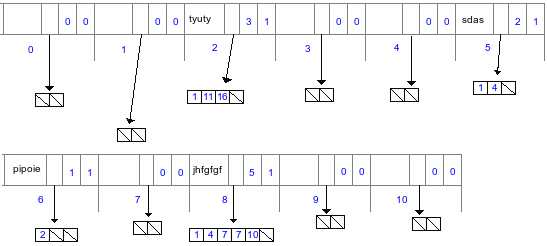
\includegraphics[scale=0.7]{hashTable_erros.jpg}\\[1cm]
\caption{Exemplo Lista de erros (Erros)}
\label{fig:minipage1}
\end{figure}
\FloatBarrier

\FloatBarrier
\subsubsection{Lista duplamente ligada (lista de linhas)}

As listas duplamente ligadas foram usadas na estrutura do Erro para conter as linhas onde certo erro ocorre. Foi usada esta estrutura pois não tem uma complexidade muito elevada (O(N), sendo N o número de linhas) e vamos ter logo as linhas ordenadas na lista pela ordem com que se encontra uma ocorrência do erro. Tentámos ainda só com arrays mas não há diferença nos tempos de execução, acabámos por optar pelas listas ligadas pois ocupam menos memória devido ao facto de crescerem dinâmicamente, a inserção tem complexidade constante, apenas a pesquisa para imprimir as linhas de cada erro tem complexidade linear, O(N), sendo N o número de linhas até um máximo de 50.  

\begin{figure}[ht]
\centering
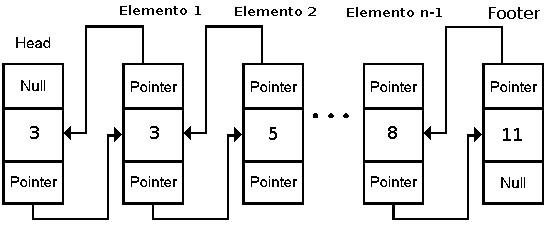
\includegraphics[scale=0.7]{listaligada.jpg}\\[1cm]
\caption{Exemplo Lista duplamente ligada (inteiros)}
\label{fig:minipage1}
\end{figure}
\FloatBarrier

\subsubsection{Cache}

A cache que temos foi feita para diminuir considerávelmente o número de acessos a disco e, consequentemente, o tempo de execução do programa de identificação e localização de erros. A cache implementada consiste em ter 2 arrays, um de blocos (hashtables) e outro de inteiros. O array de inteiros tem o mesmo número de elementos que o array de blocos e serve apenas para conter o número do bloco que está carregado numa posição da cache. Por exemplo, se quiséssemos saber se o bloco 200 se encontrava na posição 1 da cache bastava ir consultar qual o número na posição 1 do array de inteiros, se for 200 significa que o bloco 200 está já carregado na posição 1 da cache. O tamanho que definimos para a cache não é muito grande, comparativamente à quantidade de blocos que há, pois a partir de certo ponto o aumento de tempo de execução do programa passa a ser practicamente insignificante. 

\subsection{Função de Hash}

A função de hash utilizada para as hashtables foi uma vertente do djb2[1,2], um algoritmo que faz uma boa dispersão dos dados, anteriormente tinhamos outro algoritmo, uma vertente utilizando a regra de Horner, que fazia uma distribuição menos boa dos dados resultanto em mais colisões e, consequentemente, em maior tempo de execução do programa de detecção de erros. As fontes onde procurámos por estes algoritmos de hash podem ser encontradas nas referências.

\subsection{Identificação e localização de erros}

Para identificar e localizar os erros num texto que se passa como input tem-se primeiro de processar cada palavra do mesmo. 

A primeira coisa que fazemos é ler linha a linha do texto e usando um "string tokenizer" do C vamos processar palavra a palavra ( delimitadas por um espaço), caso não se chegue a um '\textbackslash n', continua a processar palavras na mesma linha, de seguida é carregado o bloco onde essa palavra esta para a cache caso não exista já na posição da cache onde se vai fazer a verificação. É fácil determinar o bloco onde se encontra uma palavra fazendo a divisão do valor de hash dessa palavra pelo número de elementos de um bloco, e, pelos testes que fizemos, vai sempre dar ao bloco correcto. Depois de se saber qual o bloco da palavra basta fazer o resto da divisão do numero do bloco pelo tamanho da cache para obtermos a posição exacta na cache onde pode estar o bloco.

Para saber se um determinado bloco está numa posição da cache temos um array de inteiros com o mesmo tamanho da cache, como já foi referido anteriormente.\\

Depois de verificar se o bloco está, ou não, na cache basta aceder directamente a posição no bloco podendo esta ser obtida a partir do resto da divisão do valor de hash da palavra pelo número de elementos de um bloco, e verificar se encontrou ou não a palavra nessa posição, caso não encontre vai tentar as seguintes até ao fim do bloco, se ainda assim não encontrar vai carregar o bloco seguinte e fazer a mesma verificação. Se mesmo assim não for encontrada vai verificar se a palavra contém alguma letra maiúscula, em caso afirmativo irá tentar procurar a palavra toda em letra minúscula da mesma maneira, carregando o bloco, indo à sua posição no bloco, procurando até ao fim e procurando no bloco seguinte. Por fim, se em letras minúsculas a palavra não for encontrada irá ser actualizado o erro caso já exista na lista de erros, incrementando as ocorrências desse erro e inserindo a linha onde ocorre na lista ligada de linhas desse erro.\\

Caso seja logo encontrada a palavra passa-se logo ao próximo token/palavra da linha que está a ser processada.\\

No fim do processamento das palavras do texto, já com a lista de erros obtidas para esse mesmo texto, é necessário ordenar a lista de erros visto que todos os elementos desta se encontram dispersos na estrutura. Para tal foi utilizado o qsort, das bibliotecas de C, que é o equivalente ao quicksort. Para usar o qsort foi necessário implementar a função de comparação para garantir que a lista de erros ficasse ordenada pelos erros que tivessem mais ocorrências e, caso tenham o mesmo número de ocorrências, pelo valor lexicográfico da palavra. Foi utilizado o quicksort para ordenar esta estrutura, não pela sua complexidade, mas pela sua performance para o número de elementos considerados para este problema (100000 ou 150000 elementos)\\

Após ordenada a lista de erros resta apenas mostrar os k erros mais frequentes (k que foi passado como argumento do programa) no standard output.

\newpage
\subsection{Complexidade}

A complexidade do programa, em geral, pelo que se pode observar é, no pior dos casos, quadrática - O(N*M) sendo N o número de palavras do texto processado e M o número de elementos de um bloco, seguindo a lógica de que para cada palavra do texto, no pior dos casos, é procurada a palavra em todas as posições do bloco e não é encontrada.\\

A complexidade do algorítmo de quicksort é quadrática (O(N²)) no número de elementos da estrutura no pior dos casos, mesmo que seja muito pouco provável que estes casos aconteçam, e logarítmica na média dos casos - O(N*log(N)), sendo N o número de elementos a ordenar, mas como a estrutura, no caso deste problema, tem poucos elementos e, segundo os testes que fizemos, é o algoritmo de ordenação mais rápido para o número máximo de elementos que vamos ter na estrutura.\\

A complexidade da função para mostrar os erros no standard output é quadrática no número de erros e número de linhas para cada erro - O(N*L) sendo N o número de erros na estrutura e L o número de linhas onde há ocorrências de um erro.\\

Quanto à inserção e pesquisa na hashtable a complexidade é constante pois este é um dos aspectos positivos acerca das hashtables - acesso directo às posições na hashtable que queremos. Por fim, relativamente às listas duplamente ligadas, apenas a pesquisa tem uma complexidade maior (linear - O(N), sendo N o número de elementos da lista), a inserção e remoção têm complexidade constante pois temos acesso direto ao header e ao footer da lista.\\ 

As restantes funções no código que fizemos têm complexidade linear (O(N)).

\newpage
\section{Conclusão}

Em conclusão achamos que conseguímos com sucesso cumprir todos os objectivos deste trabalho, e conseguimos ainda ganhar alguma experiência e agilidade com o mesmo. Tivémos alguns problemas inicialmente com a escolha da estrutura que iríamos utilizar mas fazendo uma análise do balanço entre simplicidade e eficiência (complexidade temporal) chegámos à conclusão que para este problema a estrutura mais indicada sería a HashTable.\\

Tivémos ainda outro problema relacionado com a função de hash que estávamos a utilizar anteriormente (regra de horner) que nos reduzia o tempo de execução do programa pelo simples facto de esta não estar a fazer uma boa distribuição dos elementos pela hashtable aumentando assim o número de colisões feitas. Tentámos também optimizar bastante o código que tinhamos anteriormente, poupando bastantes comparações de strings, ciclos desnecessários, condições desnecessárias/desorganizadas em if's, while's, etc.

Temos também a perfeita consciência que há bastantes aspectos no nosso código e na nossa implementação que poderiam ter sido melhorados como ter o código muito mais optimizado, ter o código muito mais organizado em bem comentado, podíamos ter usado outras estruturas mais eficientes para certos aspectos, mas achamos que, para aquilo a que nos propusémos e além dos problemas e desafios com que nos deparámos, fizemos um trabalho bastante satisfatório.

\newpage
\section{Anexos}

\subsection{Código do programa}

\textbf{\\Ficheiro: corrector.h}

\begin{verbatim}
#include "list.h"
#include "hashTableDisc.h"
#define TAMMAXPALAVRA 28
#define CAPACIDADE 2400019 // num. primo
#define NUMBLOCOS 18750 // 850021/128 = 6641 aprox
#define SIZEHT (128)  //4096/32 = 128 aproxx
#define MAXERROS 110017

char lowerCs[TAMMAXPALAVRA];

struct erro{
      char palavra[TAMMAXPALAVRA];
      LinkedList *linhas;
      int ocorrencias;
      bool usado;
};

typedef struct erro Erro;

struct listErros{
      Erro *ers;
};

typedef struct listErros listErros;

listErros* new_listErros();
void destroy_listErros(listErros*);
Erro* new_erro(char*, int);
void destroy_erro(Erro*);
int actualiza_erro(char*, int, int, listErros*);
bool find_word(char*, int, HashTable*);
int funcComp(const void *, const void *);
int choose_min(int, int);
bool isAllLower(char*);
void print_erros(int, int, listErros*);

\end{verbatim}


\textbf{\\\\\\Ficheiro: corrector.c}

\begin{verbatim}
#include <stdio.h>
#include <string.h>
#include <stdbool.h>
#include <stdlib.h>
#include <ctype.h>
#include "corrector.h"
#define M 50
#define CACHESIZE 3001

//aloca a memoria necessaria para uma lista de erros
listErros* new_listErros(){
      listErros *le = malloc(sizeof(listErros));
      le->ers = malloc(sizeof(Erro)*MAXERROS);
      memset(le->ers,0,sizeof(Erro)*MAXERROS);

      return le;
}

// liberta a memoria ocupada pela lista de erros
void destroy_listErros(listErros *le){
      free(le->ers);
      free(le);
}

//aloca memoria para um novo erro e inicializa os campos
Erro* new_erro(char *palavra, int linha){
      Erro *e = malloc(sizeof(Erro));
      strcpy(e->palavra, palavra);
      e->ocorrencias = 1;
      e->linhas = list_new();
      e->usado = true;
      list_insert(e->linhas, linha); 

      return e;
}

//liberta a memoria ocupada pelo erro
void destroy_erro(Erro *e){
      list_destroy(e->linhas);
      free(e);
}





/*procura um erro, se o encontrar actualiza-o incrementando o 
  num de ocorrencias e adicionando a linha, caso nao o encontre 
  é necessario adiciona-lo*/
int actualiza_erro(char *palavra, int h, int linha, listErros *le){
      int hv = h%MAXERROS;

      while(hv < MAXERROS){
            if(!le->ers[hv].usado)
            {	
                  /*caso nesta posicao nao esteja nada
                   e porque o erro nao existe ainda*/
                  Erro *e = new_erro(palavra, linha);
                  le->ers[hv] = *e;
                  le->ers[hv].usado = true;
                  break; 
            }

            if(le->ers[hv].usado && strcmp(le->ers[hv].palavra, palavra) == 0)
            {

                  if(le->ers[hv].ocorrencias < M)
                      list_insert(le->ers[hv].linhas, linha);
                  le->ers[hv].ocorrencias++;

                  return 0; //encontrou o erro
            }

            hv++;
            hv %= MAXERROS;
      }

      return 1;
}

/*funcao usada para procurar uma palavra num bloco*/
bool find_word(char *string, int hashVal, HashTable *tbl)
{
      int i = 0;
      int posBloco;

      // verifica se nas posições seguintes
      // do bloco la esta a palavra
      while (i < SIZEHT)
      {
            posBloco = hashVal%SIZEHT;

            if(tbl->ht[posBloco].usado == 1 && strcmp(tbl->ht[posBloco].palavra,
            string) == 0)
                return true;
            hashVal++;
            i++;
      }

      return false;
}

/*funcao de comparacao usado no qsort que ordena 2 erros 
  consoante o numero de ocorrencias e o valor da string */
int funcComp(const void *p1, const void *p2)
{
      const Erro *elem1 = p1;    
      const Erro *elem2 = p2;

      if ( elem1->ocorrencias == elem2->ocorrencias){
            if(strcmp(elem1->palavra, elem2->palavra) < 0)
                return -1;
            else
                return 1;
      }

      return (elem2->ocorrencias - elem1->ocorrencias);
}

/*verifica se uma palavra esta toda em minusculas*/
bool isAllLower(char *s){
      for(int i = 0; s[i] != '\0';i++)
            if(isupper(s[i]))
                  return false;

      return true;
}

/*Imprime os k erros encontrados e as respectivas ocorrencias*/
void print_erros(int e_enc, int k, listErros *erros)
{
      //int M = 0;
      int l_length = 0;
      int errosImp = 0;

      if(e_enc < k)
          errosImp = e_enc;
      else
          errosImp = k;

      for(int i = 0; i < errosImp; i++)
      {
            printf("%s (%d)", erros->ers[i].palavra, erros->ers[i].ocorrencias);

            //M = choose_min(erros->ers[i].ocorrencias, 50);
            l_length = list_length(erros->ers[i].linhas);

            for(int j = 0; j < l_length; j++)
                  printf(" %d", list_nth(erros->ers[i].linhas, j));

            //destroy_erro(&erros->ers[i]);

            if(i != e_enc)
                  printf("\n");
      }
}

int main(int argc,char *argv[]){
      char string[TAMMAXPALAVRA];
      char *line = NULL;
      int hashVal = 0, linha = 0;
      bool found = false;
      listErros *erros;
      int numBloco = -1, errosEnc = 0, k = 5;
      size_t len = 0;

      HashTable *cache[CACHESIZE];
      int cacheBlock[CACHESIZE];

      //inicializa a cache
      for(int i = 0; i < CACHESIZE; i++)
      {
            cache[i] = NULL;
            cacheBlock[i] = -1;
      }


      if(argc == 2)
            k = atoi(argv[1]);

      if(k>100000)
            k = 100000;

      erros = new_listErros();

      FILE *fd = fopen("dic.data","r+");

      Elemento ht;
      int hashblock = 0, tablePos = 0, choose = 0,hv = 0,scanVal = 0;
      const char s[2] = " ";
      char *token = NULL;
      int tokenlen = 0;

      while(scanVal != -1)
      {	
            if(token == NULL)
            {
                  //nova linha lida
                  scanVal = getline(&line, &len, stdin);
                  if(scanVal == -1) break;
                  token = strtok(line, s);
                  linha++;
            }

            //processamento da linha
            tokenlen = strlen(token);

            //tratar o \r
            if(tokenlen == 1 && token[tokenlen-1] == 10)
            {
                  token = strtok(NULL, s);
                  continue;
            }

            if(token[tokenlen-1] == 10)
            {
                  memcpy(string, token, tokenlen-1);
                  string[tokenlen-1] = '\0';

            }
            else
            {
                  memcpy(string, token, tokenlen);
                  string[tokenlen] = '\0';
            }

            /*calcular o hash, o bloco onde se espera estar 
              a palavra e o bloco da cache a procurar*/
            hashVal = hash(string);	
            hashblock = hashVal/SIZEHT;
            choose = (hashblock % CACHESIZE);
            //printf("cache block: %d\n", choose);
            tablePos = hashVal%SIZEHT;
            if(cache[choose] == NULL)
            {
                  cache[choose] = new_HT();
            }

            if(hashblock != cacheBlock[choose])
            {
                  carregar_bloco(cache[choose], fd, hashblock);
                  cacheBlock[choose] = hashblock;
              //	printf("cache block loaded: %d\n", choose);
            }

            ht = cache[choose]->ht[tablePos];

            if(ht.usado == 0 || strcmp(ht.palavra, string) != 0){

                  found = find_word(string, hashVal, cache[choose]);

                  if(!found || tablePos == SIZEHT-1){
                        carregar_bloco(cache[choose], fd, hashblock+1);
                        cacheBlock[choose] = hashblock+1;

                        //caso nao tenha sido encontrada tentar as restantes
                        //posicoes do bloco
                        found = find_word(string, hashVal+1, cache[choose]);
                  }

                  if(!found){
                        //caso nao esteja no bloco tentar em lower case caso
                        // a palavra nao esteja toda em lower case
                        if(!isAllLower(string)){	
                              //e necessario memset para evitar lixo

                              memset(lowerCs,0, sizeof(char)*TAMMAXPALAVRA);

                              for(int i = 0; string[i]!='\0'; i++){
                                    lowerCs[i] = tolower(string[i]);
                              }

                              hv = hash(lowerCs);
                              numBloco = hv/SIZEHT;
                              choose = (numBloco % CACHESIZE);
                      //		printf("cache block: %d\n", choose);
                              tablePos = hashVal%SIZEHT;

                              if(cache[choose] == NULL)
                              {
                                    cache[choose] = new_HT();
                              }

                              // recarrega o bloco para a cache caso 
                              // nao encontre a palavra na cache
                              if(cacheBlock[choose] != numBloco)
                              {
            carregar_bloco(cache[choose], fd, numBloco);
            cacheBlock[choose] = numBloco;
            //			printf("cache block loaded: %d\n", choose);
                                    }

            ht = cache[choose]->ht[tablePos];	

            if(ht.usado == 0 || strcmp(ht.palavra, lowerCs) != 0){

            found = find_word(lowerCs, hv, cache[choose]);

            if(!found) {
                //conta quantos erros novos sao inseridos
                errosEnc += actualiza_erro(string, hashVal, linha, erros);

            }	
          }
        }
        else
              errosEnc += actualiza_erro(string, hashVal, linha, erros);
      }

    }

    token = strtok(NULL, s);
  }

  qsort(erros->ers, MAXERROS, sizeof(Erro), funcComp);
  //quicksort(erros->ers);

  print_erros(errosEnc, k, erros);

  fclose(fd);

  destroy_listErros(erros);

  for(int i = 0; i < CACHESIZE; i++)
  {
  		destroy_HT(cache[i]);
  }

  return 0;
}
\end{verbatim}

\textbf{\\\\\\\\\\\\\\\\Ficheiro: hashTableDisc.h}

\begin{verbatim}
#include <stdio.h>
#include <string.h>
#include <stdbool.h>
#include <stdlib.h>
#define TAMMAXPALAVRA 28
#define CAPACIDADE 2400019 // num. primo
#define NUMBLOCOS 18750 // 850021/128 = 6641 aprox
#define SIZEHT (128)  //4096/32 = 128 aproxx
	
struct elemento{
      char palavra[TAMMAXPALAVRA];
      int usado;
};

typedef struct elemento Elemento;

struct hashtable{
      Elemento *ht; 
};

typedef struct hashtable HashTable;

unsigned int hash(char *);
HashTable* new_HT();
void destroy_HT(HashTable*);
void carregar_bloco(HashTable*, FILE *, int);
void escreve_elem(Elemento, FILE *fd);
void criar_dic(char *,int);
bool pesquisa_Elem(char *nomeFicheiro, char *);
void insere_dados(FILE *, int, char *);
\end{verbatim}

\newpage

\textbf{Ficheiro: hashTableDisc.c}

\begin{verbatim}
#include "hashTableDisc.h"

//devolve o valor de hash duma string

/*calcula o hash de uma string
  Algoritmo de hashing usado -> djb2

  http://www.cse.yorku.ca/~oz/hash.html  */

unsigned int hash(char *string){
	
      unsigned int hash = 5381;
      int c;

      while ((c = *string++))
            hash = ((hash << 5) + hash) + c; 

      hash %= CAPACIDADE;

      return hash;
}

/*carrega um bloco do dicionario em disco 
  para a hashtable em memória*/
void carregar_bloco(HashTable* ht, FILE *fd, int pos)
{
      fseek(fd, pos*SIZEHT*sizeof(Elemento), SEEK_SET);
      fread(ht->ht, SIZEHT*sizeof(Elemento), 1, fd);
}

/*aloca memoria necessaria para uma hashtable (bloco)*/
HashTable* new_HT()
{
      HashTable *ht = malloc(sizeof(HashTable));
      ht->ht = malloc(sizeof(Elemento)*SIZEHT);
      memset(ht->ht,0,sizeof(Elemento)*SIZEHT);

      return ht;
}

/*liberta a mem ocupada pela hashtable (bloco)*/
void destroy_HT(HashTable *ht)
{
      if(ht == NULL) return;
      free(ht->ht);
      free(ht);
}

/* cria um novo dicionario com um nome e 
   um tamanho (numero de elementos)*/
void criar_dic(char *nomeFicheiro,int tamanho)
{

      FILE *fd;
      Elemento elem;
      
      //inicializar elemento da hashtable a 0
      memset(&elem,0,sizeof(Elemento)); 

      fd = fopen(nomeFicheiro,"w");

      if(fd == NULL)
      {
            perror("Erro: criar_tabela - fopen.");
            exit(0);
      }

      for(int i=0;i<tamanho;i++)
      {
            fwrite(&elem,sizeof(Elemento),1,fd);
      }
      
      fclose(fd);
}

/*pesquisa um elemento em disco*/
bool pesquisa_Elem(char *nomeFicheiro, char *string)
{
      FILE *fd = fopen(nomeFicheiro, "r+");
      Elemento tmp;
      int pos = hash(string);

      while(1){
            fseek(fd, pos*sizeof(Elemento), SEEK_SET);
            fread(&tmp, sizeof(Elemento), 1, fd);

            if (tmp.usado == 0){
                  fclose(fd);
                  return false;	
            }

            if (tmp.usado == 1 && strcmp(tmp.palavra, string) == 0){
                  fclose(fd);
                  return true;
            }

            //printf("Colisao!\n");
            pos++;
            pos = pos%CAPACIDADE;
      }

      fclose(fd);

      return false;

}

/*insere um elemento na hashtable criada em disco*/
void insere_elemento(FILE *fd, int chave, char *string)
{
      /* elemento a inserir (elem) e temporario(tmp) para 
          pesquisar o ficheiro e verificar se o ficheiro 
          a inserir ja existe na hash table*/
      Elemento elem, tmp;
      int pos = chave;	

      elem.usado = 1;
      strcpy(elem.palavra, string);


      if(fd == NULL)
      {
            perror("Erro: insere_dados - fopen.");
            exit(0);
      }

      //procura por uma posição não usada para inserir
      while(1)
      {
            fseek(fd, pos*sizeof(Elemento), SEEK_SET);
            fread(&tmp, sizeof(Elemento), 1, fd);	
            if (tmp.usado == 0)
                  break;
            //printf("Colisao!\n");
            pos++;
            pos %= CAPACIDADE;
      }

      //printf("pos = %d\n", pos);
      fseek(fd, pos*sizeof(Elemento), SEEK_SET);
      fwrite(&elem, sizeof(Elemento),1,fd);
	
}

\end{verbatim}

\textbf{Ficheiro: list.h}

\begin{verbatim}
/*
  ########################################################
 #####     Exercicios EDAII - linked lists header     #####
  ########################################################
 */

typedef struct Node Node;
typedef struct LinkedList LinkedList;

LinkedList *list_new();
Node *node_new();
bool list_empty(LinkedList *list);
bool list_insert(LinkedList *list, int value);
bool list_remove(LinkedList *list, int value);
int list_length(LinkedList *list);
void list_print(LinkedList *list);
int list_find(LinkedList *list, int value);
void list_destroy(LinkedList *list);
int list_nth(LinkedList *list, int n);

#########################################################################
\end{verbatim}

\textbf{Ficheiro: list\_double.c}

\begin{verbatim}

/*
  ########################################################
 ##### Exercicios EDAII - Listas simplesmente ligadas #####
  ########################################################
 */

#include <stdio.h>
#include <stdlib.h>
#include <stdbool.h>
#include "list.h"

//double linked lists

typedef struct Node{  // nó de uma lista ligada

      int elem;         //um elemento inteiro
      struct Node *next;       //O proximo nó na lista
      struct Node *prev;       //O nó anterior na lista

} Node;

typedef struct LinkedList{  //uma lista duplamente ligada de nós

      struct Node *head;
      struct Node *tail;
      int size;

} LinkedList;

//cria e inicializa uma nova lista duplamente ligada 
LinkedList *list_new(){    //aloca e inicializa a lista com NULL's 

      //aloca o espaco necessario para a lista
      LinkedList *list = malloc(sizeof(LinkedList));  

      // inicializa a lista com tamanho 0 e null na cabeca
      list -> head = NULL;
      list -> tail = NULL;
      list -> size = 0;

      return list;
}

//cria e inicializa um novo nó
Node *node_new(){
      Node *node = malloc(sizeof(Node));
      node -> next = NULL;
      node -> prev = NULL;
      return node;
}

//verifica se a lista esta vazia
bool list_empty(LinkedList *list){
      return list -> size == 0;  
}

//insere um elemento à cauda da lista
bool list_insert(LinkedList *list, int value){
      Node *node;

      node = node_new();
      node -> elem = value;

      if(list -> tail == NULL){
            // se a lista estiver vazia a cabeca e a cauda passam a ser
            // o nó com o elemento que se prentende inserir	
            list -> tail = node;
            list -> head = node; 
      }

      else{
            // insere no fim da lista, a cauda passa a ser o novo no
            list -> tail -> next = node;
            node -> prev = list -> tail;
      }

      list -> tail = node;
      list -> size++;
      return true;
}

// remove um elemento da lista
bool list_remove(LinkedList *list, int value){
      Node *current;

      current = list -> head;

      //percorre a lista ate encontrar o elemento 
      while(current != NULL && current -> elem != value)
            current = current -> next;


      if (list -> size != 0 && current != NULL){

            /* se o valor se encontrar na posicao 0, ou seja,
             se estiver à cabeca é removido*/
            if(current == list -> head){
                  current = list -> head;

                  // o elemento que esta a cabeca passa a ser o proximo da cabeca
                  list -> head = current -> next;
                  
                  // a cabeça fica sem nó anterior
                  current -> next -> prev = NULL; 
            }
            /*se o valor estiver no fim da lista, ou seja,
             se estiver na cauda é removido*/
            else if(current == list -> tail){
                  current = list -> tail;

                  // o elemento anterior da cauda fica sem nó seguinte
                  current -> prev -> next = NULL;
                  
                  // a cauda passa a ser o elemento anterior a antiga cauda
                  list -> tail = list -> tail -> prev;
            }		

            /*caso o valor se encontrar entre a cabeça e a cauda*/
            else{
                  //coloca o nó anterior ao actual
                  //como anterior do proximo do actual
                  current -> next -> prev = current -> prev;

                  //coloca o nó seguinte ao actual 
                  //como o seguinte do anterior do nó actual
                  current -> prev -> next = current -> next;
            }

            list -> size--;
            free(current);
            return true;
      }

      return false;
}

// verifica se encontra o valor na lista
int list_find(LinkedList *list, int value){
      Node *current = list -> head;
      int i = 0; // indice

      while(current != NULL){
            //se encontrar o valor no nó actual devolve a sua posicao
            // caso contrario continua a percorrer a lista
            if(current -> elem == value)
                  return i;

            else{
                  current = current -> next;
                  i++;
            }
      }

      return -1;
}

// devolve o tamanho da lista
int list_length(LinkedList *list){
      return list -> size;
}

// imprime uma representação da lista para a consola
void list_print(LinkedList *list){
      Node *current = list -> head;

      printf("[");

      //percorre a lista ate ao fim imprimindo cada elemento
      while(current!=NULL){
            printf("%d", current -> elem);

            if (current -> next != NULL){
                  printf(" ");	
            }

            current = current -> next;
      }

      printf("]");
}

// liberta todo o espaço em memória ocupado pela lista 
void list_destroy(LinkedList *list){
      Node *previous, *current = list -> head;
      //liberta a memoria de cada no da lista
      while(current -> next != NULL){
            previous = current;
            current = current -> next;
            free(previous);
      }
      free(current);

      //liberta a memoria da lista
      free(list);
}

// pesquisa o n-ésimo elemento da lista
int list_nth(LinkedList *list, int n){
      Node *current;
      int i = 0; // indice

      /*comeca a verificar a partir da cabeça
        ou da cauda de acordo com o n*/
      if (n < (list -> size) /2 -1){
            current = list -> head;

            //percorre a lista ate encontrar o elemento 
            for(i=0; i<n; i++)
                  current = current -> next;

      }
      /*comeca a verificar a partir da cauda*/
      else{
            current = list -> tail;

            //percorre a lista ate encontrar o elemento 
            for(i= (list -> size)-1; i> n; i--)
                  current = current -> prev;
      }

      return current -> elem;	
}
#########################################################################
\end{verbatim}

\textbf{Ficheiro: criacao.c}

\begin{verbatim}
#include <stdio.h>
#include <string.h>
#include <stdbool.h>
#include <stdlib.h>
#include "hashTableDisc.h"
#define TAMMAXPALAVRA 28
#define CAPACIDADE 2400019 // num. primo
#define NUMBLOCOS 18750 // 2400019/128 = 18750 aprox
#define SIZEHT (128)  //4096/32 = 128 aproxx

/*############## Criacao dicionario ########################*/

int main(void){
      int chave = 0;

      criar_dic("dic.data",CAPACIDADE);

      char string[TAMMAXPALAVRA];

      FILE* fd = fopen("dic.data","r+");
      int scanVal = 0;
      while(scanVal != EOF)
      {

            for(int i=0;i<TAMMAXPALAVRA;i++)
                  string[i]=0;

            scanVal = fscanf(stdin, "%s",string);
            chave = hash(string);
            insere_elemento(fd, chave, string);		
      }

      fclose(fd);
      return 0;
}
\end{verbatim}

%\includegraphics[width=0.5\textwidth]{diagrama.jpg}
%\caption{\label{fig:diagrama}This is a figure caption.}
%\end{figure}


%\begin{figure}[!htbp]
%  \caption{Como é efectuado o login do lado do servidor.}
%  \centering
%    \includegraphics[width=0.7\textwidth]{NovoServidorLogin.jpg}
%\end{figure}

\begin{thebibliography}{9}
  
\bibitem{lamport94}
  York University,
  \emph{"Hash Functions"}. \\$http://www.cse.yorku.ca/\sim oz/hash.html$

\bibitem{lamport94}
  StackExchange,
  \emph{"Which hashing algorithm is best for uniqueness and speed?"}. $http://programmers.stackexchange.com/questions/49550/which-hashing-algorithm-is-best-for-uniqueness-and-speed$

\end{thebibliography}


\end{document}